\section{Conclusions and Future Work}

\begin{frame}{Content Overview}
    \footnotesize
    \begin{enumerate}
        \item \textcolor{gray!50}{Motivation, Background, and Objectives}
        \item \textcolor{gray!50}{Addressing the Impossible Trinity of Modeling (ITM)}
        \item \textcolor{gray!70}{Unified Control-Theoretic Training}
        \item \textcolor{gray!50}{Addressing the Impossible Trinity of Optimal Control (ITOC)}
        \item \colorbox{yellow!70}{\textbf{Conclusions and Future Work}}
    \end{enumerate}
\end{frame}

\begin{frame}{Conclusions and Future Work}
    \footnotesize
    \visible<1->{Contributions are made to resolving the \textbf{ITM} with improved \textbf{generalizability},}
    \begin{columns}
        \begin{column}{0.6\textwidth}
            \only<1>{
                \begin{figure}
                    \centering
                    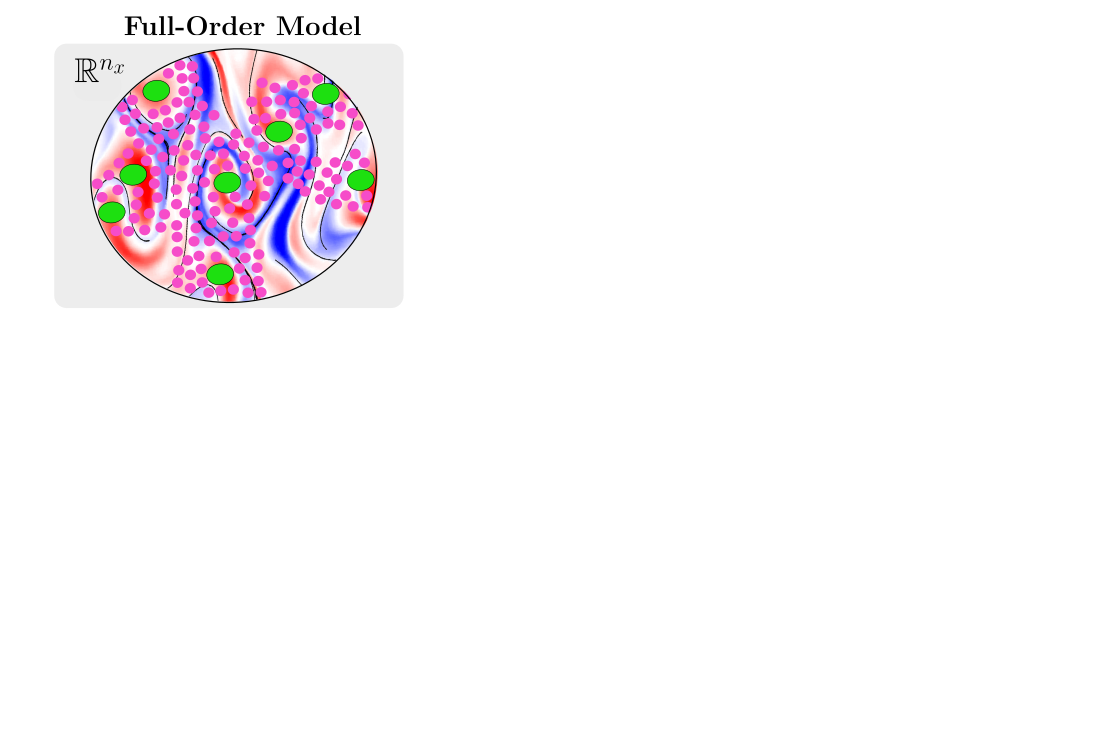
\includegraphics[width=0.99\textwidth]{../figs/conclusions/conclusion_overview_1.png}
                \end{figure}}
            \only<2>{
                \begin{figure}
                    \centering
                    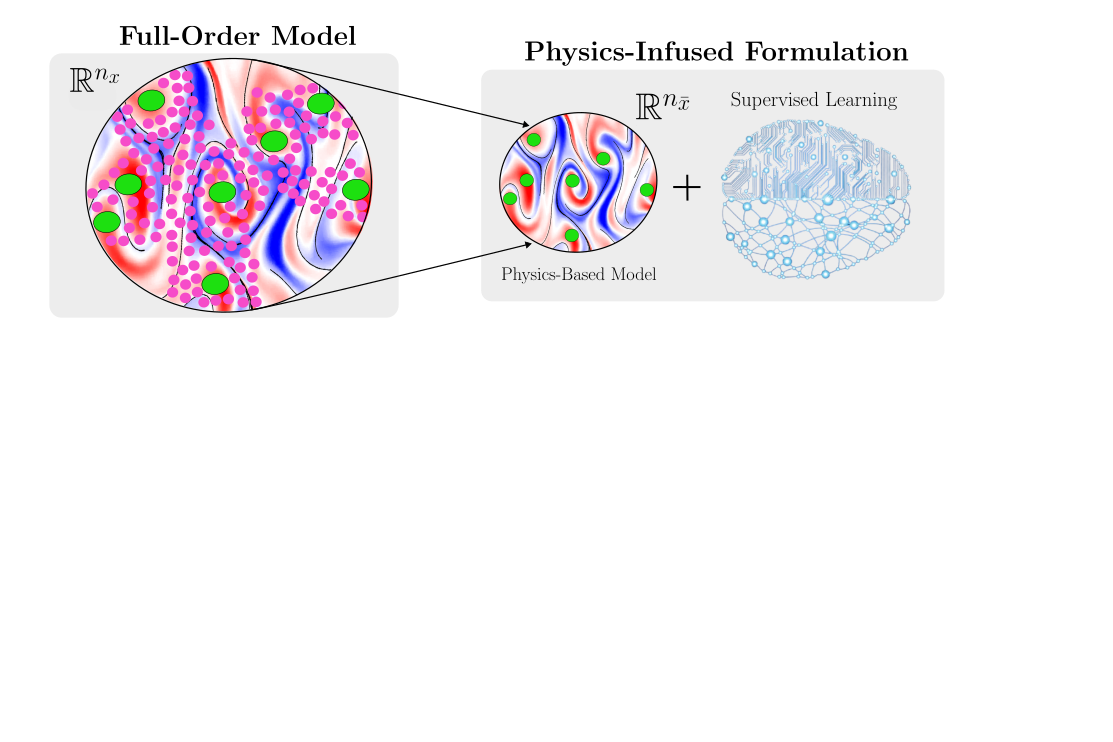
\includegraphics[width=0.99\textwidth]{../figs/conclusions/conclusion_overview_2.png}
                \end{figure}}
            \only<3>{
                \begin{figure}
                    \centering
                    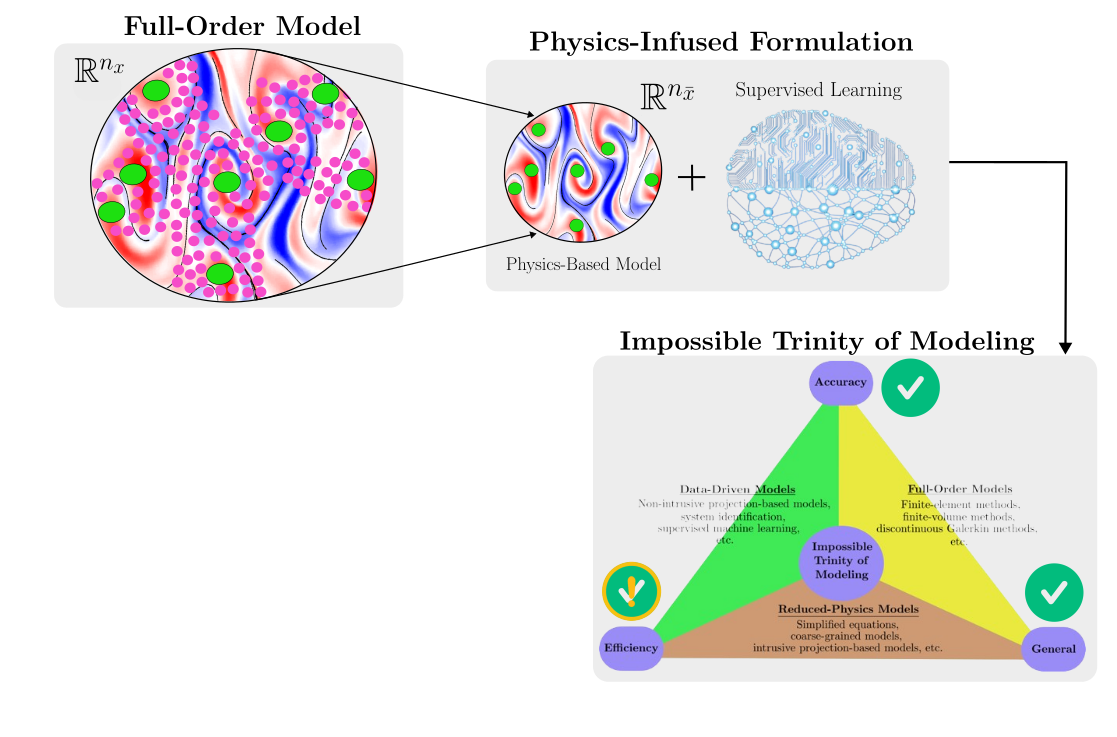
\includegraphics[width=0.99\textwidth]{../figs/conclusions/conclusion_overview_3.png}
                \end{figure}}
            \only<4>{
                \begin{figure}
                    \centering
                    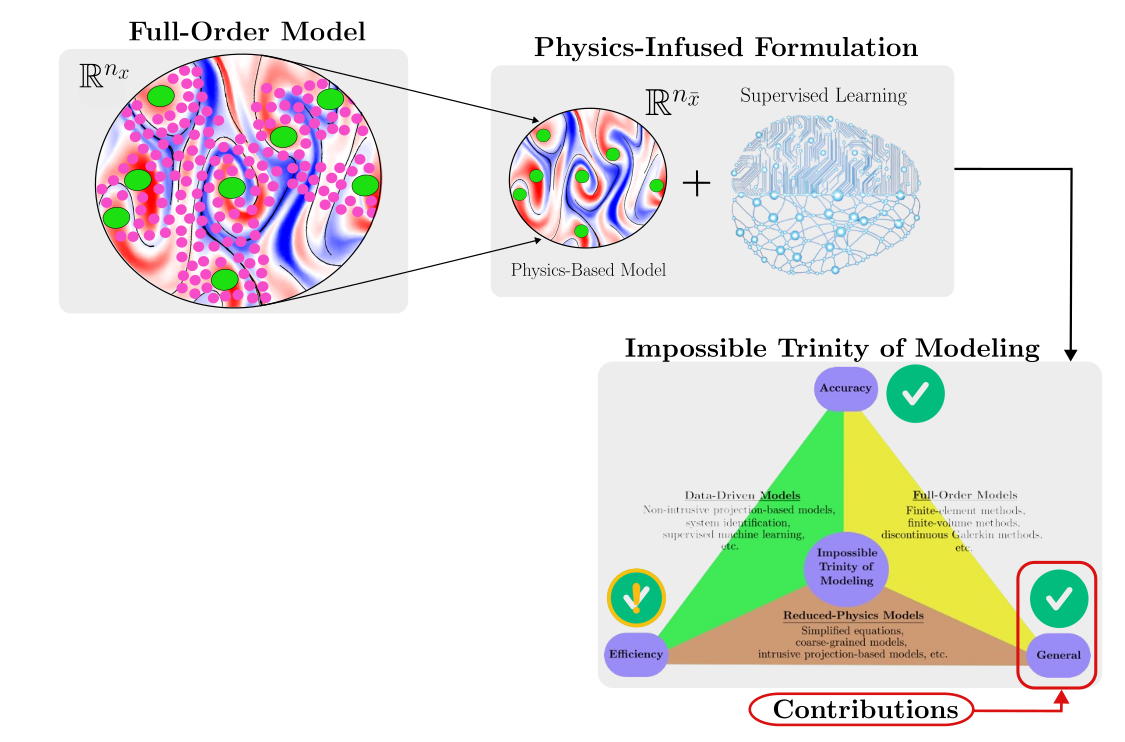
\includegraphics[width=0.99\textwidth]{../figs/conclusions/conclusion_overview_4.png}
                \end{figure}}
            \only<5>{
                \begin{figure}
                    \centering
                    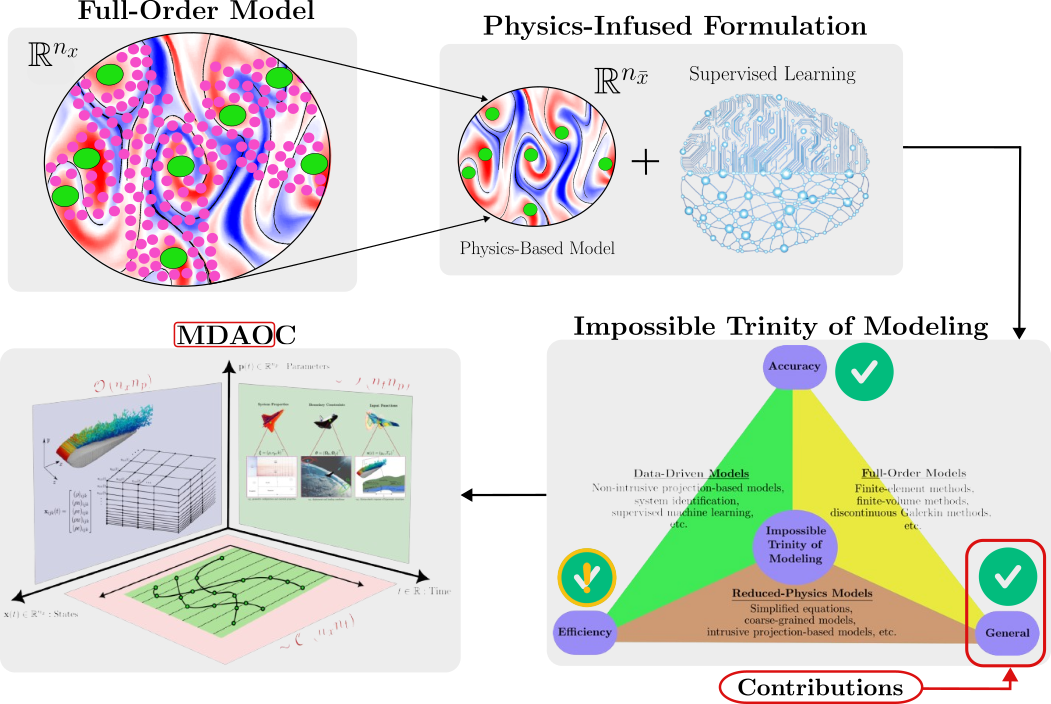
\includegraphics[width=0.99\textwidth]{../figs/conclusions/conclusion_overview_5.png}
                \end{figure}}
            \only<6->{
                \begin{figure}
                    \centering
                    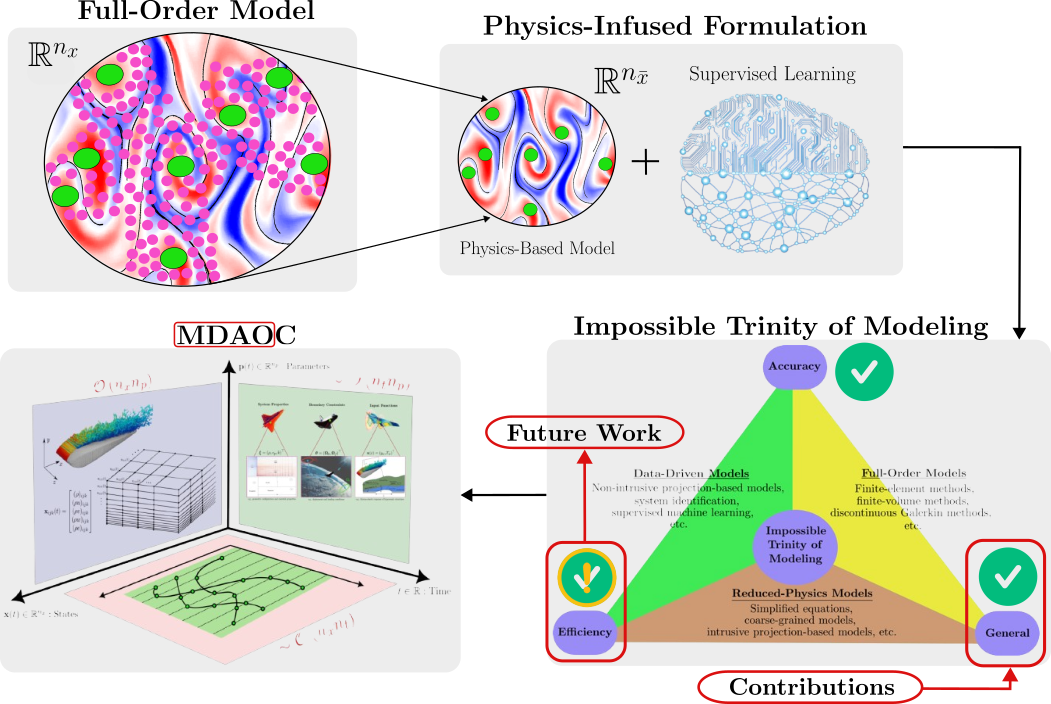
\includegraphics[width=0.99\textwidth]{../figs/conclusions/conclusion_overview_6.png}
                \end{figure}}
        \end{column}
        \begin{column}{0.4\textwidth}
            \tiny
            \visible<4->{
            \begin{graybox}{Main Contributions}
                \begin{itemize}
                    \item \textcolor{red}{\textbf{Systematic approach}} to physics infusion
                    \item Improved \textcolor{red}{\textbf{generalizability}}
                \end{itemize}
            \end{graybox}}
            \visible<6->{
            \begin{graybox}{Future and On-going Work}
                \begin{itemize}
                    \item<7-> Training overheads are still large \textcolor{red}{\textbf{(similar to neural ODE)}},
                    \item<8-> \textcolor{red}{\textbf{Learning from sparse noisy observables}} (on-going work),
                    \item<9> \textcolor{red}{\textbf{Apply PIROM to more complex multi-physical settings}} (e.g., on-going work on ablating hypersonic TPS).
                \end{itemize}
            \end{graybox}}
        \end{column}
    \end{columns}
\end{frame}

\begin{frame}{Conclusions and Future Work}
    \footnotesize
    \visible<1->{Contributions to resolving the \textbf{ITOC} are made with improved \textbf{efficiency} and \textbf{generalizability},}
    \begin{columns}
        \begin{column}{0.6\textwidth}
            \only<1>{
                \begin{figure}
                    \centering
                    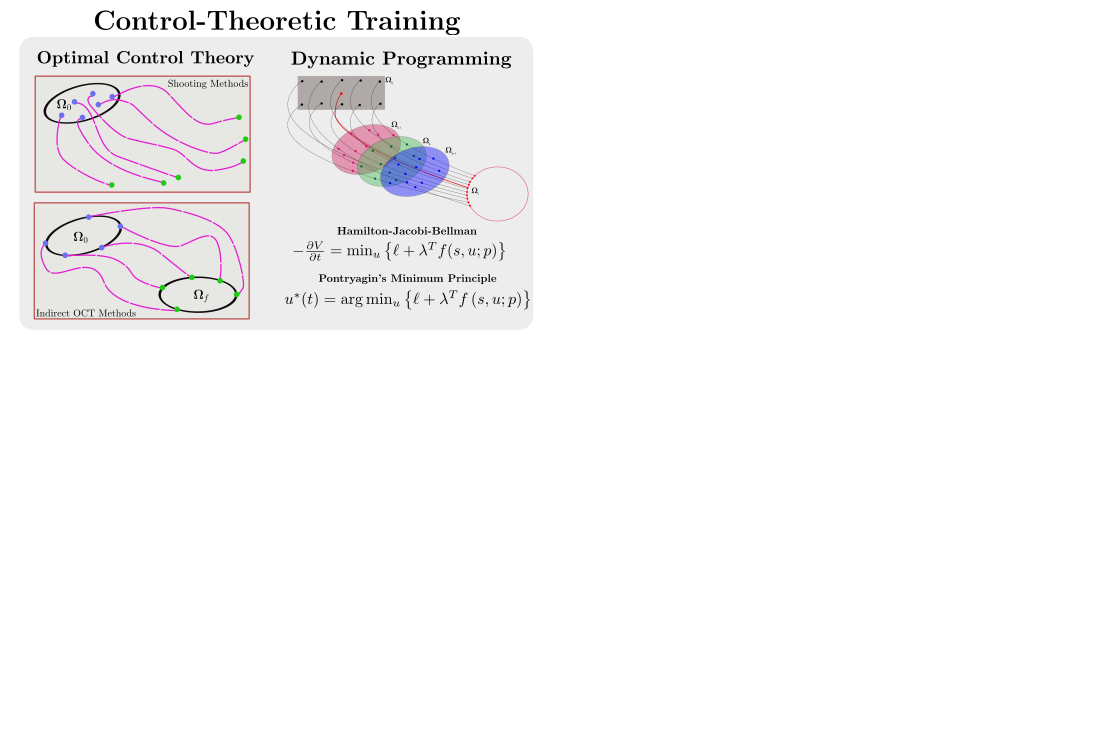
\includegraphics[width=0.99\textwidth]{../figs/conclusions/control_overview_1.png}
                \end{figure}}
            \only<2>{
                \begin{figure}
                    \centering
                    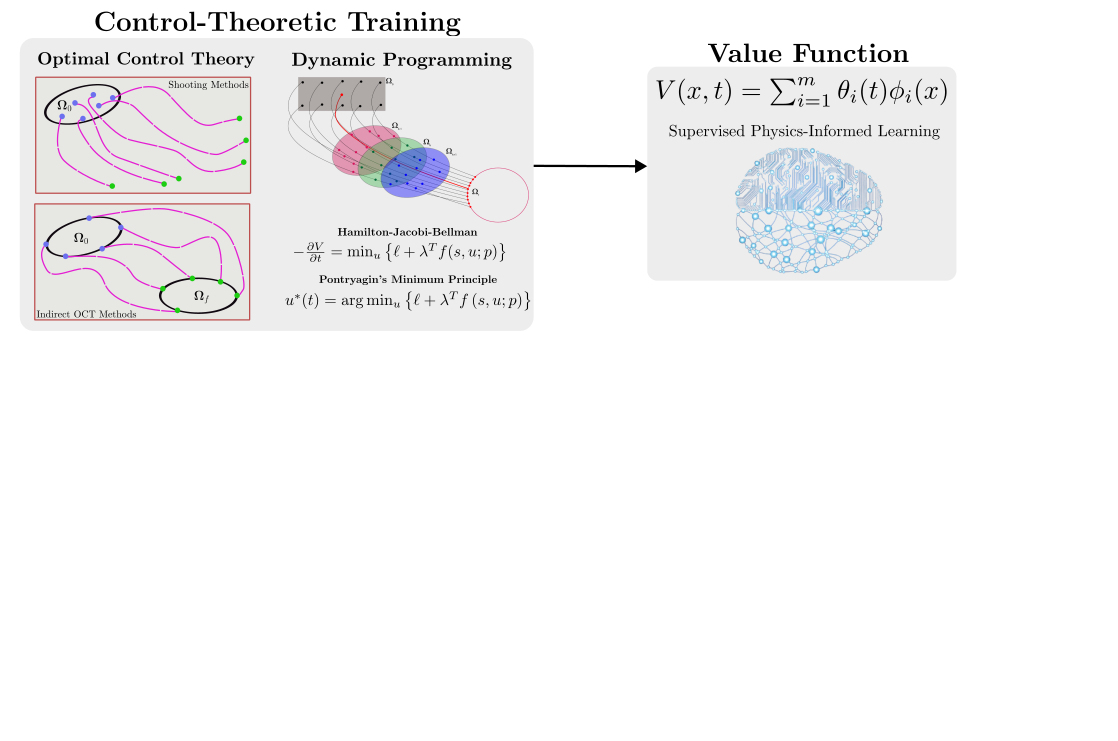
\includegraphics[width=0.99\textwidth]{../figs/conclusions/control_overview_2.png}
                \end{figure}}
            \only<3>{
                \begin{figure}
                    \centering
                    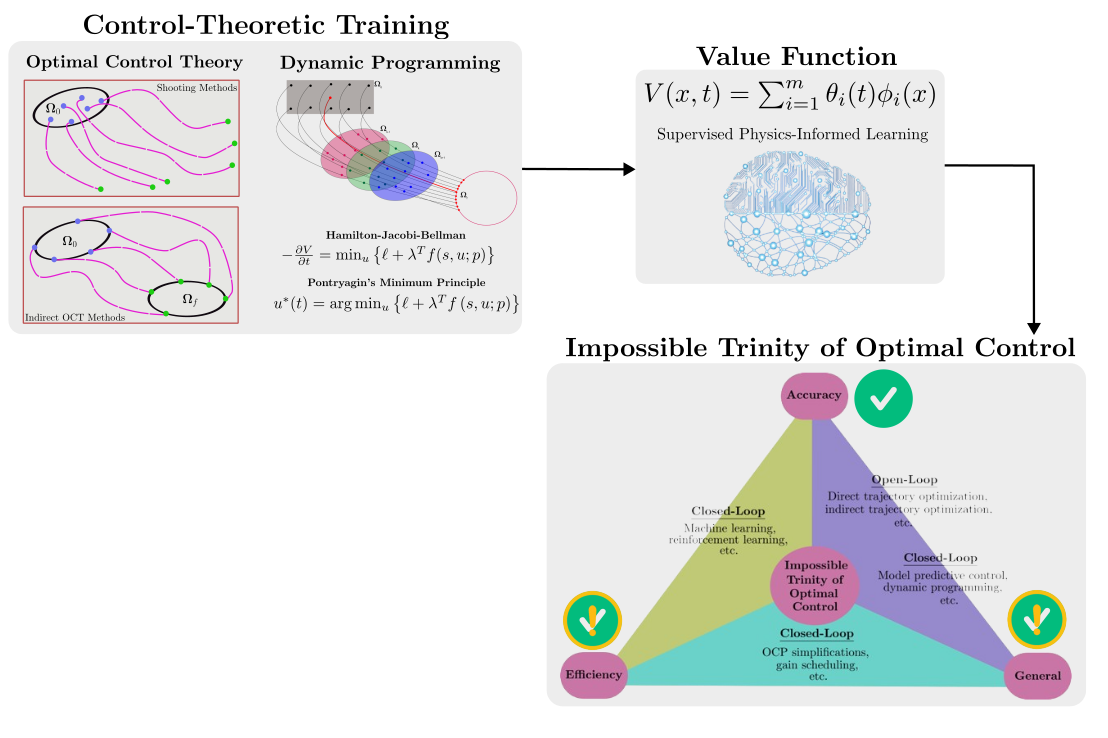
\includegraphics[width=0.99\textwidth]{../figs/conclusions/control_overview_3.png}
                \end{figure}}
            \only<4>{
                \begin{figure}
                    \centering
                    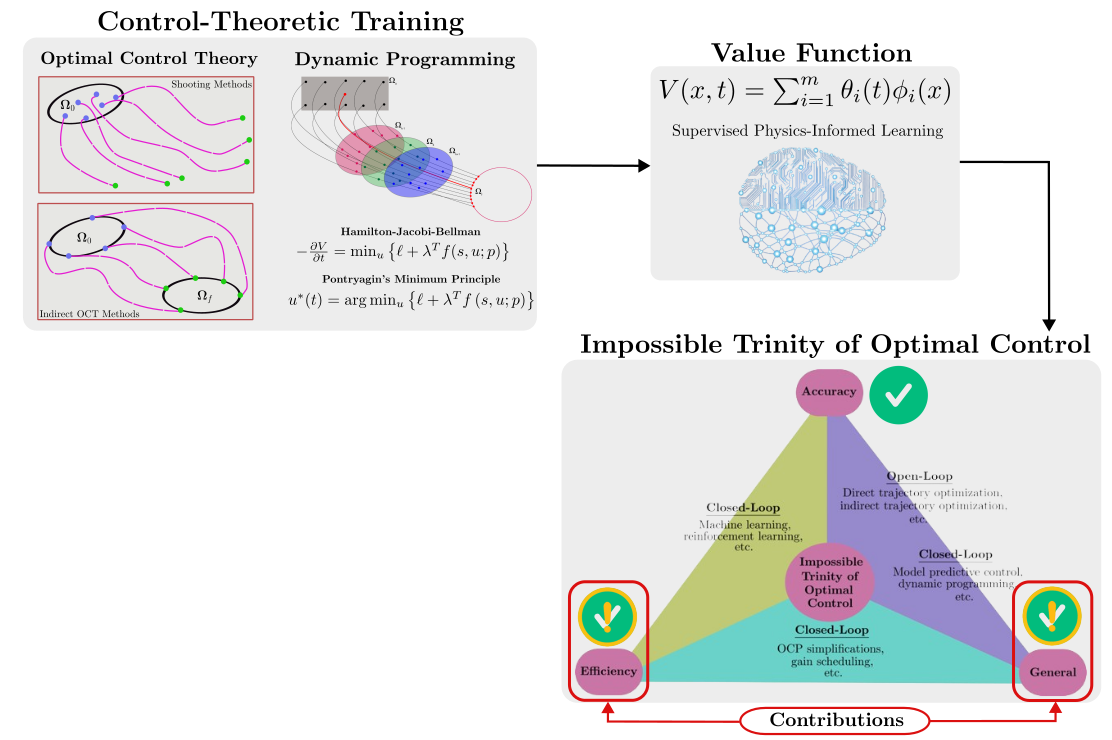
\includegraphics[width=0.99\textwidth]{../figs/conclusions/control_overview_4.png}
                \end{figure}}
            \only<5>{
                \begin{figure}
                    \centering
                    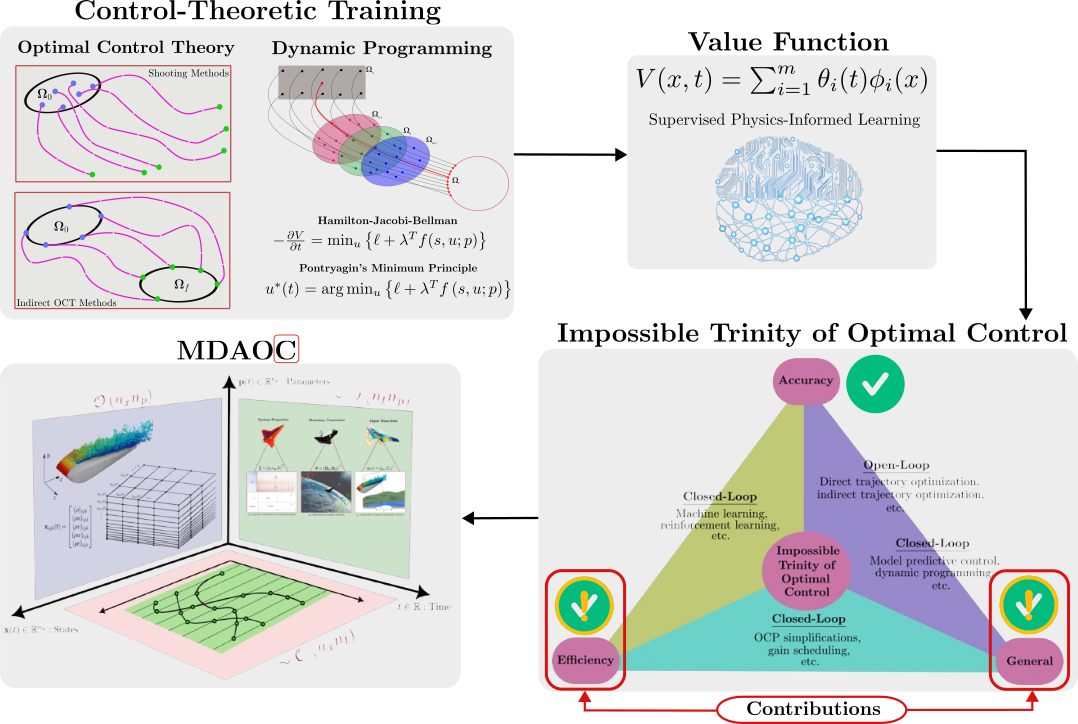
\includegraphics[width=0.99\textwidth]{../figs/conclusions/control_overview_5.png}
                \end{figure}}
            \only<6->{
                \begin{figure}
                    \centering
                    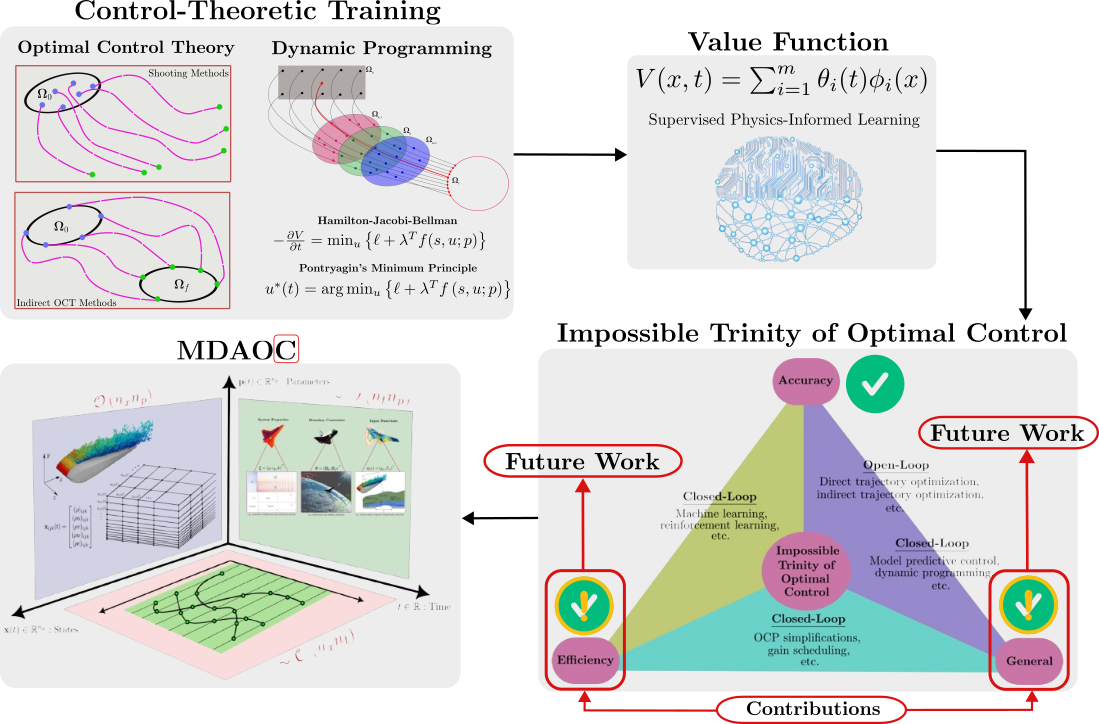
\includegraphics[width=0.99\textwidth]{../figs/conclusions/control_overview_6.png}
                \end{figure}}
        \end{column}
        \begin{column}{0.4\textwidth}
            \tiny
            \visible<4->{
            \begin{graybox}{Main Contributions}
                \begin{itemize}
                    \item<4-> \textcolor{red}{\textbf{Improved generalizability}} relative to costate-based optimal closed-loop control,
                    \item<4-> \textcolor{red}{\textbf{Improved efficiency}} through compressed sensing for low-memory deployment in embedded systems
                \end{itemize}
            \end{graybox}}
            \visible<6->{
            \begin{graybox}{Future and On-going Work}
                \begin{itemize}
                    \item<7-> \textcolor{red}{\textbf{Develop one-step learning}} of value function for faster training,
                    \item<8-> \textcolor{red}{\textbf{Guarantee robustness}} to unknown model perturbations via \textcolor{red}{\textbf{robust control}} methods,
                \end{itemize}
            \end{graybox}}
        \end{column}
    \end{columns}
\end{frame}

\begin{frame}{Publications}
    \tiny
    \textbf{Journal papers}:
    \begin{itemize}
        \item \textbf{Carlos A. Vargas Venegas}, Daning Huang, Puneet Singla, Sean Nolan, and Michael Grant. ``Sparse Physics-Informed Learning Via Dynamic Programming for Optimal Feedback Control''. \emph{arXiv pre-print} (under review).
        \item \textbf{Carlos A. Vargas Venegas}, Daning Huang, Patrick Blonigan, and John Tencer. ``Physics-Infused Reduced-Order Modeling for Analysis of Multi-Layered Hypersonic Thermal Protection Systems''. \emph{Structural and Multidisciplinary Optimization}. 2025. (Accepted).
        \item \textbf{Carlos A. Vargas Venegas}, Puneet Singla, Michael J. Grant, Maruthi Akella, and Manoranjan Majji. ``Parsimonious Parametrization of Hypersonic Vehicle Trajectories for a Given Domain of Mission Variables''. \emph{Journal of DoD Research and Engineering (JDR\&E)}. 2024. (Accepted).
        \item \textbf{Carlos A. Vargas Venegas} and Daning Huang. ``Physics-Infused Reduced-Order Modeling of Hypersonic Aerothermal Loads for Aerothermoelastic Analysis''. \textit{AIAA Journal}. Volume 61. Number 3. 2022.
    \end{itemize}
    \textbf{Conference papers}:
    \begin{itemize}
        \item \textbf{Carlos A. Vargas Venegas}, Daning Huang, Patrick Blonigan, and John Tencer. ``Physics-Infused Reduced-Order Modeling for Analysis of Multi-Layered Non-Decomposing Ablating Hypersonic Thermal Protection Systems''. In \emph{AIAA SciTech 2026}, January 2026.
        \item \textbf{Carlos A. Vargas Venegas} and Daning Huang. ``Development of Weak-Form Physics-Infused Reduced-Order Modeling With Applications''. In \emph{AIAA SciTech 2024}, January 2024.
        \item Mihir Vedantam, \textbf{Carlos A. Vargas Venegas}, Damien Gueho, Puneet Singla, and Maruthi R. Akella. ``On-Board Optimal Feedback Controller Generation for Hypersonic Re-Target Scenarios''. In \emph{AIAA SciTech 2023}, January 2023.
        \item \textbf{Carlos A. Vargas Venegas} and Daning Huang. ``Physics-Infused Reduced-Order Modeling of Hypersonic Aerothermal Loads for Aerothermoelastic Analysis''. In \emph{AIAA SciTech 2022}, January 2022.
        \item \textbf{Carlos A. Vargas Venegas} and Daning Huang. ``Expedient Hypersonic Aerothermal Prediction for Aerothermoelastic Analysis via Field Inversion and Machine Learning''. In \emph{AIAA SciTech 2021}, January 2021.
    \end{itemize}
\end{frame}

\begin{frame}{References}
    \tiny
    [1] Carlos A. Vargas Venegas and Daning Huang. ``Physics-Infused Reduced-Order Modeling of Aerothermal Loads for Hypersonic Aerothermoelastic Analysis''. \emph{AIAA Journal}. Volume 61. Number 3. 2022. DOI: 10.2514/1.J062214.\newline
    [2] Eric Parish and Karthik Duraisamy. ``Coarse-Graining Turbulence Using the Mori-Zwanzig Formalism''. \emph{Cambridge University Press. 2025}. DOI: 10.1017/9781009377379\newline
    [3] Yin Yu, John Harlim, Daning Huang, and Yan Li. ``Learning Coarse-Grained Dynamics on Graph''. \emph{Physica D: Non-Linear Phenomena}. Volume 481, 2025: DOI: 10.1016/j.physd.2025.134801.\newline
    [4] Ricky T. Q. Chen, Yulia Rubanova, Jesse Bettencourt, and David K. Duvenaud. ``Neural Ordinary Differential Equations''. \emph{Advances in Neural Information Processing Systems 31 (NeurIPS 2018)}. 2018. DOI: 10.48550/arXiv.1806.07366. \newline
    [5] Michael Mercurio, ``Sparse collocation Methods for Solving High-Dimension PDEs in Estimation and Control of Dynamical Systems''. \emph{Ph.D. thesis, State University of New York at Buffalo}. 2017. 
    [6] Dimitri P. Bertsekas. ``Dynamic Programming and Optimal Control''. \emph{Athena Scientific}, 2004.
\end{frame}

\begin{frame}{Acknowledgements}
    \footnotesize
    \begin{columns}
        \begin{column}{0.3\textwidth}
            \begin{figure}
                \centering
                
\includegraphics[width=0.45\textwidth]{../figs/acknowledgments/penn_state_logo.png}
            \end{figure}
            \begin{figure}
                \centering
                
\includegraphics[width=0.45\textwidth]{../figs/acknowledgments/snl_logo.png}
            \end{figure}
        \end{column}
        \begin{column}{0.7\textwidth}
            {\tiny
            This work was supported by Sandia National Laboratories through the year-round internship program. Sandia National Laboratories is a multi-mission laboratory managed and operated by National Technology \& Engineering Solutions of Sandia, LLC (NTESS), a wholly owned subsidiary of Honeywell International Inc., for the U.S. Department of Energy's National Nuclear Security Administration (DOE/NNSA) under contract DE-NA0003525. This written work is authored by an employee of NTESS. The employee, not NTESS, owns the right, title and interest in and to the written work and is responsible for its contents. Any subjective views or opinions that might be expressed in the written work do not necessarily represent the views of the U.S. Government. The publisher acknowledges that the U.S. Government retains a non-exclusive, paid-up, irrevocable, world-wide license to publish or reproduce the published form of this written work or allow others to do so, for U.S. Government purposes. The DOE will provide public access to results of federally sponsored research in accordance with the DOE Public Access Plan.}
        \end{column}
    \end{columns}
\end{frame}